\documentclass[a4paper, 11pt]{article}
\usepackage[utf8]{inputenc} 
\usepackage[T1]{fontenc}
\usepackage[top=2cm,bottom=2cm,left=2cm,right=2cm]{geometry}
\usepackage{graphicx}
\usepackage[french]{babel}
\usepackage{multirow,multicol}
\usepackage{amsmath, amssymb, latexsym}
\usepackage{pstricks,pst-node,pst-coil,pst-grad,pst-plot}
\usepackage{epsfig,subfigure}
\usepackage[lined,boxed]{algorithm}
\usepackage{algorithmic}
\usepackage{sectsty}
\usepackage{xcolor}

\usepackage{url}

\usepackage{setspace}

\newtheorem{definition}{Definition}
\newtheorem{example}{Example}
\newtheorem{proposition}{Proposition}
\newtheorem{proof}{Proof}

\definecolor{color_section}{RGB}{87,68,95}
\definecolor{color_subsection}{RGB}{46,81,159}
\definecolor{color_sub-subsection}{RGB}{121,142,200}

\sectionfont{\color{color_section}\underline}
\subsectionfont{\color{color_subsection}\underline}
\subsubsectionfont{\color{color_sub-subsection}\underline}

\begin{titlepage}


\title{- Rapport de projet - \\ Conception d'un jeu Tetris}
\author{\textsc{André} Lorada  (21809742) \\ \textsc{Lebranchu} Paul  (21403460) \\ \textsc{Levesque} Willy  (21808901)  \\ \textsc{Lopez-pardo} Hugues  (21803489) }
\date{Avril 2019}

\end{titlepage}
\begin{document}

    \begin{titlepage}
        \begin{figure}[t]
            
\includegraphics[scale=1]{images/logo.png}
        \end{figure}
        
        \maketitle
        
        \thispagestyle{empty}
    \end{titlepage}

    \newpage
    \tableofcontents

    \newpage
    \section{Introduction}
        %Paul-Lorada
        Le projet que nous devions réaliser était la conception d'un Tetris du début à la fin, en python en utilisant la bibliothèque Pygame. Le Tetris devait contenir un mode multijoueurs, qui peut s'effectuer de différentes manières: 
        
        \begin{itemize}
            \item soit deux joueurs sur le même ordinateur
            \item soit un joueur contre une IA
            \item soit deux joueurs sur deux ordinateurs, chacun ayant leurs propres interfaces (réseau).
        \end{itemize}
        
        De nombreuses fonctionnalités devaient être implantées comme les fonctionnalités de base du Tetris (la création d'une grille, des Tetrominos, le déplacement de ceux-ci, un score,...) et des fonctionnalités spécifiques au mode multijoueurs, comme le fait d'ajouter une ligne de malus à l'adversaire lorsque nous réalisons une ligne par exemple.
        \newline
        Pour pouvoir réaliser cela, nous pouvions nous baser sur les nombreuses versions de Tetris qui ont existé à travers le temps. Il y eu de nombreuses évolutions des mécanismes de jeu du Tetris entre la première version de Tetris, sortie sur Gameboy en 1989 et la dernière version : Tetris 99 sortie en février 2019 (où 99 joueurs s'affrontent dans une "battle royale" de Tetris : le but étant d'être le dernier survivant).
        \newline
        Dans un premier temps, nous avons décidé de nous inspirer d'un tutoriel que nous avons trouver sur Youtube (le lien est dans les sources) pour avoir une idée de comment réaliser un Tetris sur Pygame avant de nous lancer dans notre propre version du Tetris. Nous allons maintenant vous expliquer le déroulement de la conception du jeu de Tetris.
        
    %#########################################################################
    \newpage
    \section{Organisation du projet}
        %------------------------------------------------------------------------
        \subsection{Gestion du projet}
            %Lorada
            Pour mener à bien ce projet, nous avons utilisé différents outils permettant de bien s'organiser sur le projet. Pour cela, on a utilisé subversion (SVN) afin de facilité la coopération du groupe, ainsi que la gestion des différentes versions du projet.
            
            \begin{figure}[ht]
                \centering
                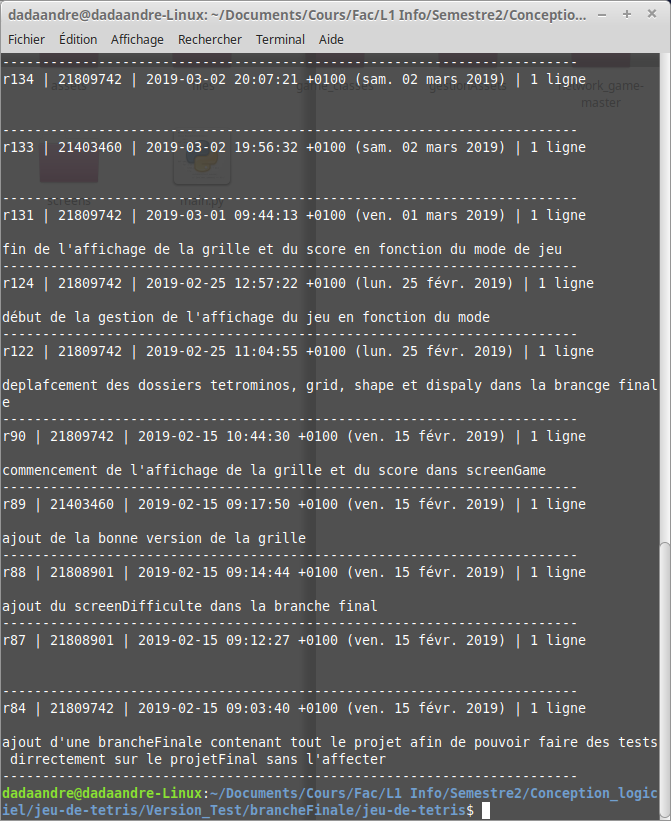
\includegraphics[scale=0.25]{images/svnLog.png}
                \caption{Extrait des différentes révisions du projet sur SVN}
            \end{figure}
            
            Afin de faciliter la gestion du projet, nous avons utilisé "Forge" d'Unicaen qui permet de créer et d'administrer des dépôts SVN très facilement par l'intermédiaire d'une interface web. D'autres fonctionnalités sont disponibles comme une gestion des permissions, une visualisation des différents commits, visualiser l'activité du projet, etc.
            
             \begin{figure}[h]
                \centering
                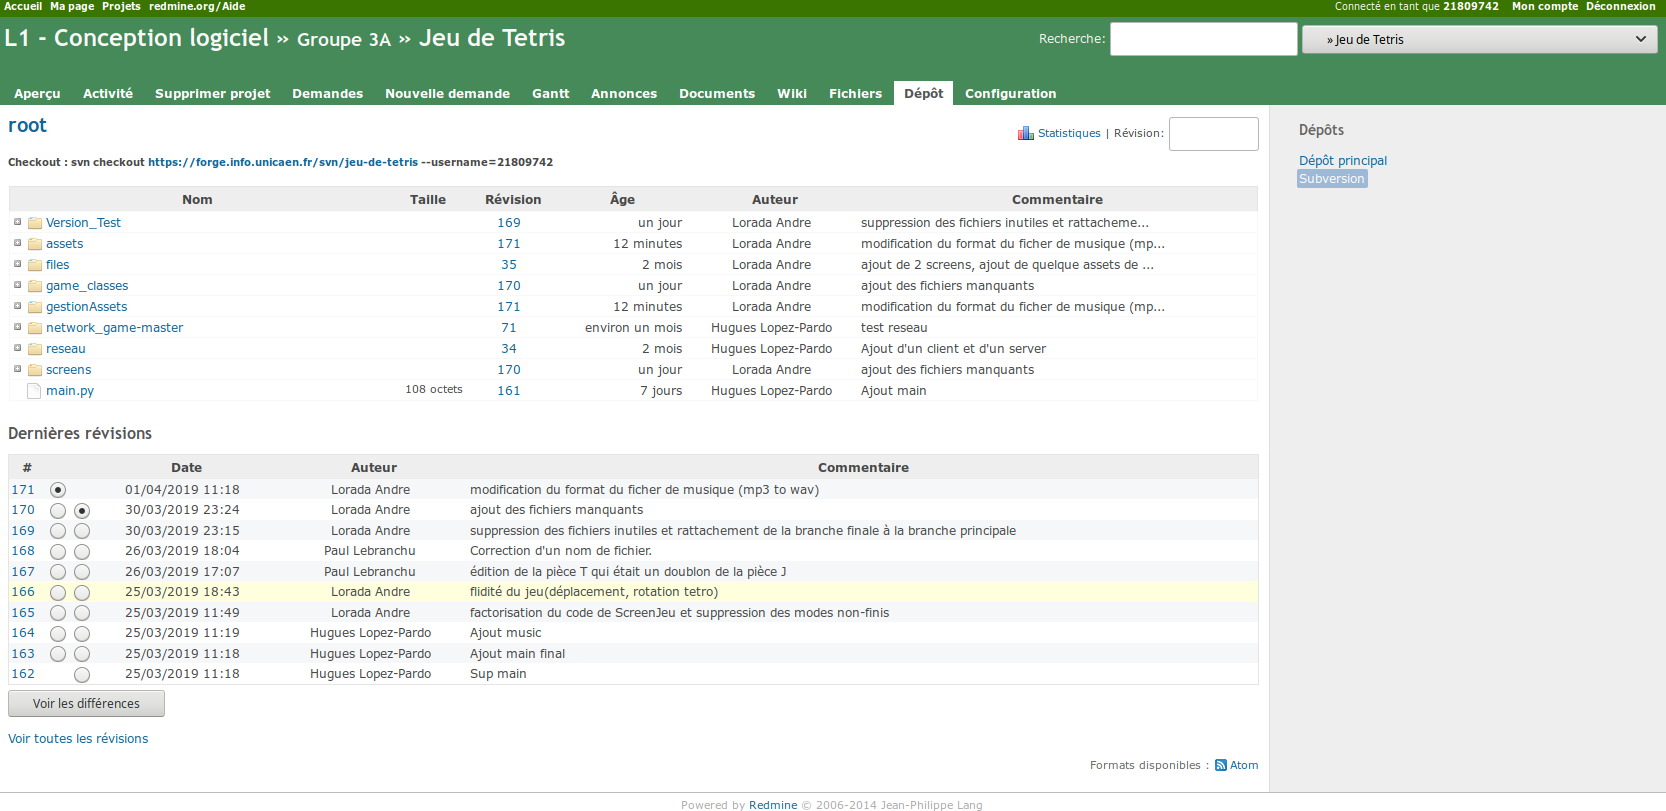
\includegraphics[scale=0.25]{images/forge.png}
                \caption{interface de Forge}
            \end{figure}
            
            Pour déterminer ce que chacun d'entre nous avait à réaliser dans le projet, nous avons décomposé celui-ci en différentes tâches afin d'avoir une vision du projet dans sa globalité. Nous avons utilisé pour cela Trello. Nous avons catégorisé certaines tâches en y ajoutant des "étiquettes" telles que "important", "priorité basse", etc.
            \newpage
            \begin{figure}[ht]
                \centering
                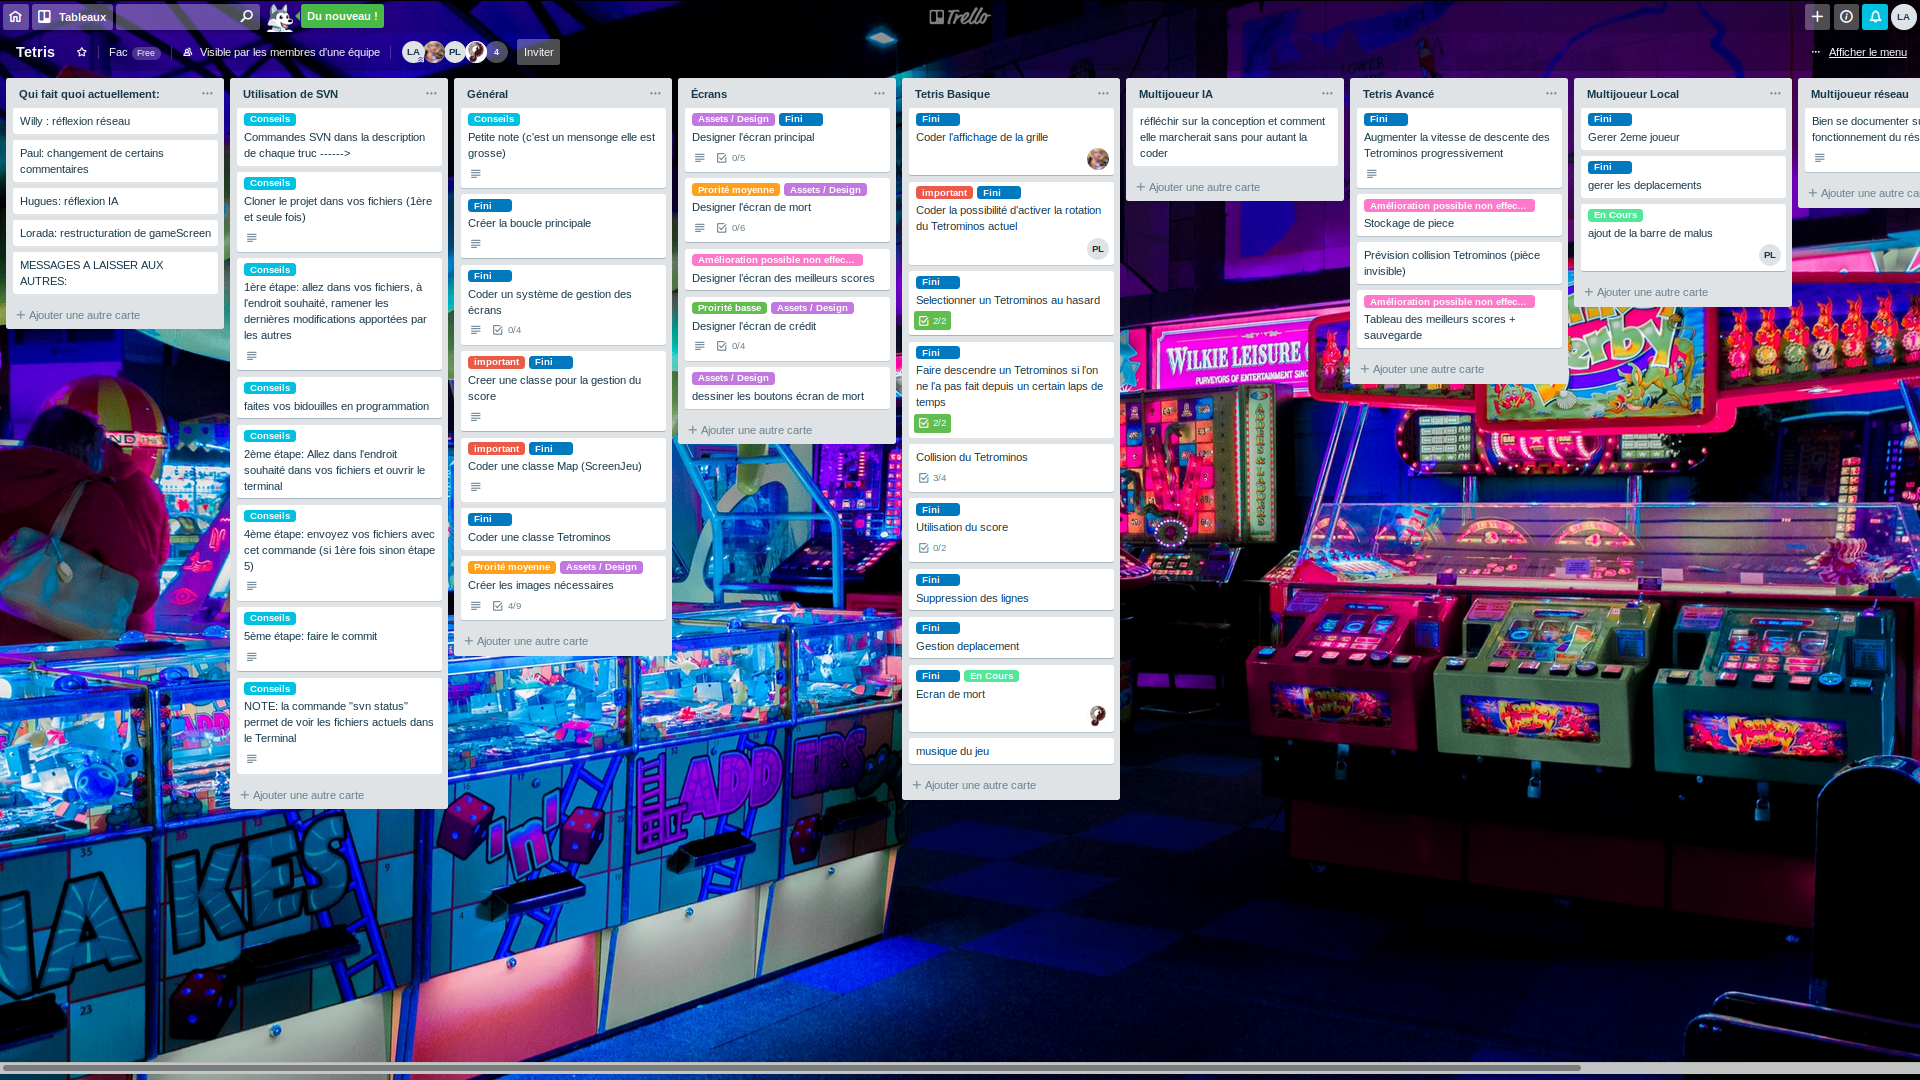
\includegraphics[scale=0.2]{images/trello.png}
                \caption{Capture d'écran du tableau sur Trello}
            \end{figure}
            
            De manière générale, lorsqu'une personne avait effectué une modification importante, une correction d'un bug, ou d'autres changements, il le signalait sur Discord (une messagerie instantanée, du même principe que Skype) pour faciliter la communication.
            
            \begin{figure}[ht]
                \centering
                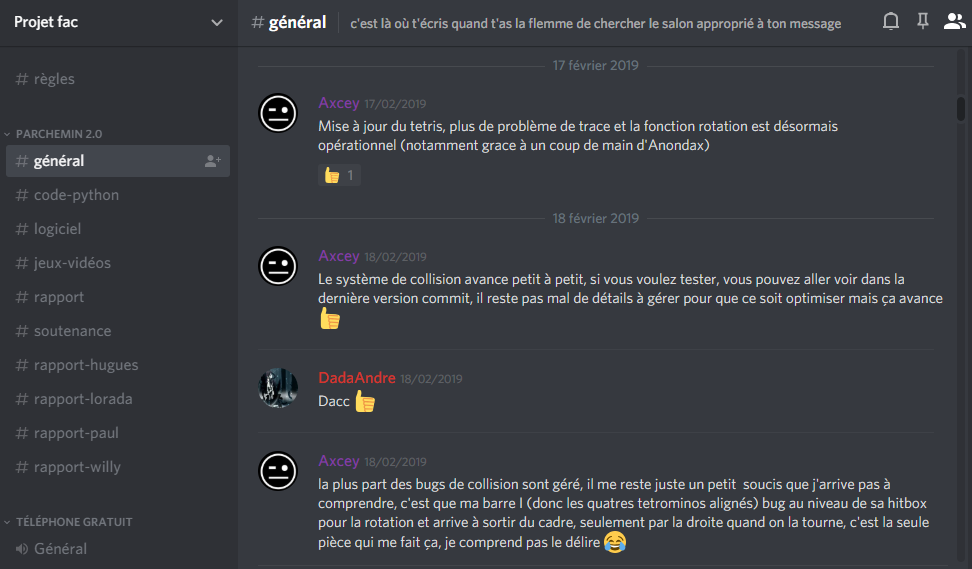
\includegraphics[scale=0.5]{images/discord.png}
                \caption{Extrait des messages sur Discord}
            \end{figure}
            
       %------------------------------------------------------------------------ 
        \subsection{Répartition des tâches}
            %Paul
            Pour concevoir le Tetris, la répartition des tâches était indispensable. A l'origine les tâches étaient réparties en deux équipes de la manière suivante:
            \begin{itemize}
                \item Une équipe était chargé de créer l'interface graphique du jeu (la gestion des écrans du menu et l'intégration du code du jeu).Cette équipe devait également se charger de trouver des pistes afin de pouvoir jouer en réseau. L'équipe était composé de Willy et de Lorada.
                \item L'autre équipe était chargé de programmer le jeu (création des classes de la grille de jeu, des pièces et du jeu en lui-même). Cette équipe devait également se charger de trouver des pistes pour programmer une IA pour le jeu. Cette équipe était composé de Paul et de Hugues.
            \newline
            \end{itemize}
            %Lorada
            Finalement, la répartition du travail s'est déroulé de la manière suivante:
            
            \begin{itemize}
                \item - Paul a codé le coeur du jeu: la création des Tetrominos, la sélection de ceux-ci de manière aléatoire, la gestion de la grille, la rotation des Tetrominos, toutes les collisions des Tetrominos (entre eux, contre les "murs de la grille"), la suppression d'une ligne et l'ajout d'une ligne de malus.
                \item Lorada a codé un système d'écran qui permet de passer du menu principal à l'écran de jeu facilement et sans mélanger tout les codes, le système de score et niveau, la réadaptation du code dans le projet final (transformer des codes procéduraux en code objet), l'affichage du jeu en fonction du mode de jeu choisi par l'utilisateur, une classe pour utiliser facilement des boutons pour le menu, ainsi que la conception d'une partie du menu.
                \item Hugues s'est chargé d'utiliser un code d'un Tetris existant comme aide pour la conception du projet. Il a fallu transformer ce code en objet, cependant cette tâche n'aboutissant pas, la décision fût prise de recommencer de zéro le projet, sans utiliser le code existant. Il s'est occupé de l'affichage de la grille. Il s'est également chargé de la réflexion sur le fonctionnement de l'IA et son implémentation.
                \item Willy s'est chargé de la réflexion sur le réseau ainsi que de quelques écrans de menu du jeu.
            \end{itemize}
       
            \underline{Organisation du temps:}
            %Paul
            \begin{itemize}
            	\item \underline{11 janvier 2019:} Début du projet Tetris, création de la Forge, du Trello et du Discord. Répartition des tâches et création des équipes.
            	\item \underline{semaine du 14 au 20 janvier:} Création des premiers dossiers/fichiers du projet et étude de la documentation Pygame de façon individuelle.
            	\item \underline{semaine du 21 au 27 janvier:} Première version du Tetris, fortement inspiré du tutoriel que nous avions trouvé sur Youtube. 
            	\item \underline{semaine du 28 janvier au 3 février:} Début du travail sur l'interface graphique (Lorada), étude approfondi du code de Youtube et début de notre propre code du jeu (Hugues/Paul).
            	\item \underline{semaine du 4 au 10 février:} Ajout des premiers boutons du menu (Lorada), première version de la grille du jeu et premières fonctionnalités implantées (Hugues/Paul).
            	\item \underline{semaine du 11 au 17 février:} Redémarrage à zéro du code du jeu, création de la classe Grid (Paul), premières pistes pour l'intelligence artificielle (Hugues) et initialisation de la classe Tetrominos (Paul),et de la classe Shape (Paul).
            	\item \underline{semaine du 18 au 24 février:} Création de nombreuses fonctionnalités du jeu: mise à jour de la classe Grid, Tetrominos et du fichier Shapes(Paul).
            	%détail un peu plus vu tout ce qui tu a fait cette semaine là
            	\item \underline{semaine du 25 février au 3 mars:} Optimisation du code du jeu (notamment de la collision des pièces) et ajout des dernières fonctionnalités (la ligne de malus)(Lorada/Paul), gestion du score(Lorada), du niveau(Lorada) et pistes pour une version du jeu en réseau (Willy).Affichage de l'interface de jeu en fonction du mode(Lorada), gestion du mode un joueur et deux joueurs(Lorada), de leur indépendance de gameplay (touches différentes, gestion des différents scores, ...)(Lorada) et d'affichage dans la classe "ScreenJeu"(Lorada). Sélection du mode de jeu dans le menu principal(Lorada).
            	\item \underline{semaine du 4 au 10 mars:} Correction des derniers bugs concernant la collision des Tetrominos et gestion de 	l'affichage des scores dans tout les modes de jeu (Lorada). Rattachement des classes ("Grid" principalement) à "ScreenJeu" (Lorada)
            	\item \underline{semaine du 11 au 17 mars:} Fin de la gestion de la fonctionnalité de la ligne de malus pour la version de test (Paul), pistes pour l'intelligence artificielle (Hugues), gestion de l'écran de mort (Lorada/Willy).
            	\item \underline{semaine du 18 au 24 mars:} Gestion de la ligne de malus aléatoire dans le dossier finale, factorisation du code (Lorada).
            	\item \underline{semaine du 25 au 31 mars:} Gestion de la musique du jeu (Hugues),fin de la factorisation du code et suppression des fichiers inutiles (Lorada), débats sur certains aspects techniques du code (faut-il plutôt un code très factorisé qui souffre de quelques ralentissements ou un code moins factorisé mais qui ne souffre pas de ses ralentissements?) et début de la rédaction du rapport.
            	\item \underline{du 1\ier{} au 15 avril:} Rédaction du rapport, préparation pour la soutenance et dernières modifications des fichiers du jeu (édition des commentaires du code, réglages de quelques bugs). Création de la classe "ScreenAmelioration" pour les modes non-développés (Lorada)
            
            \end{itemize}
            
            Voici un graphique représentant le nombre de commits effectué sur Forge durant le projet. Nous pouvons observer que le travail est réparti de façon équitable entre les mois de janvier, février et mars.
            
            \begin{figure}[ht]
                \centering
                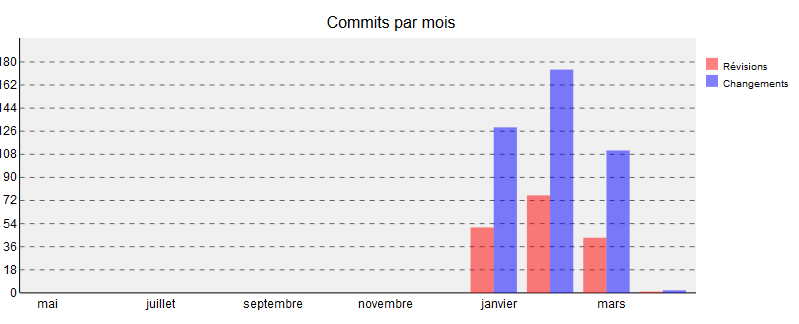
\includegraphics[scale=0.5]{images/Commit.png}
                \caption{Graphique sur les commits}
            \end{figure}
    %############################################################################ 
    \section{Architecture du projet}
        %------------------------------------------------------------------------
        \subsection{Arborescence du projet}
        %Lorada
            Sur subversion, le projet est organisé de manière suivante: 
            \begin{figure}[ht]
                \centering
                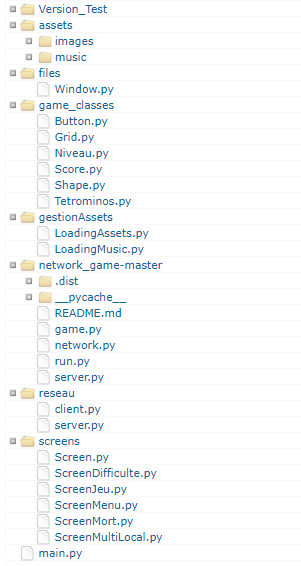
\includegraphics[scale=0.75]{images/arborescence.png}
                \caption{Arborescence du projet sur Forge}
            \end{figure}
            On y retrouve: 
            \begin{itemize}
                \item Un dossier Version\_Test, qui comprenait toute les classes qui étaient en cours de conception. Lorsque celles-ci étaient fonctionnelles, elles étaient remises dans la version finale du jeu, Ce procédé était utile afin que les autres membres du projet puissent programmer sur d'autres fonctionnalités sans que les modifications d'une personne ait un impact sur le travail de tout le monde (par exemple la modification d'une classe dont un autre personne en est dépendante).
                \item un dossier "assets", qui concentre toute les ressources du jeu (images et musique).
                \item un dossier "files" contenant Window.py. Cette classe, se charge d'afficher la fenêtre du jeu, la boucle du jeu ainsi que la transition entre deux écrans.
                \item un dossier "game\_classes", regroupant toute les autres classes du projet, qui corespondent chacunes d'entre elles à un élément du jeu (un bouton, une grille, un Tetrominos, etc.)
                \item un dossier "gestionAssets", qui contient deux classes, permettant de simplifier le chargement des ressources (images et musique) dans le jeu.
                 \item un dossier "network\_game\_master" et un dossier "réseau" qui constituent les tests pour le jeu en réseau.
                \item un dossier "screen", regroupant les différentes classes qui gèrent les écrans du jeu. 
                
            \end{itemize}
        
        %-------------------------------------------------------------------------
        \subsection{Diagramme des modules et des classes}
        %Lorada
            Pour lancer le jeu, le fichier "main.py" doit être éxécuté". Une fois lancé, celui-ci fait appel à la classe "Window" (contenu dans le fichier Window.py), qui se chargera d'appeler à son tour la classe "ScreenMenu" (contenu dans le fichier ScreenMenu.py). La classe "ScreenMenu" (qui hérite de la classe Screen) s'occupera de l'affichage du contenu du premier écran du menu principal. L'ensemble des écrans du menu du jeu ont essentiellement besoin des classes "LoadingAssets", permettant de charger les images du jeu et de "Button", qui est une classe ayant pour fonction de créer les boutons du jeu.
            
            \begin{figure}[ht]
        		\centering
        			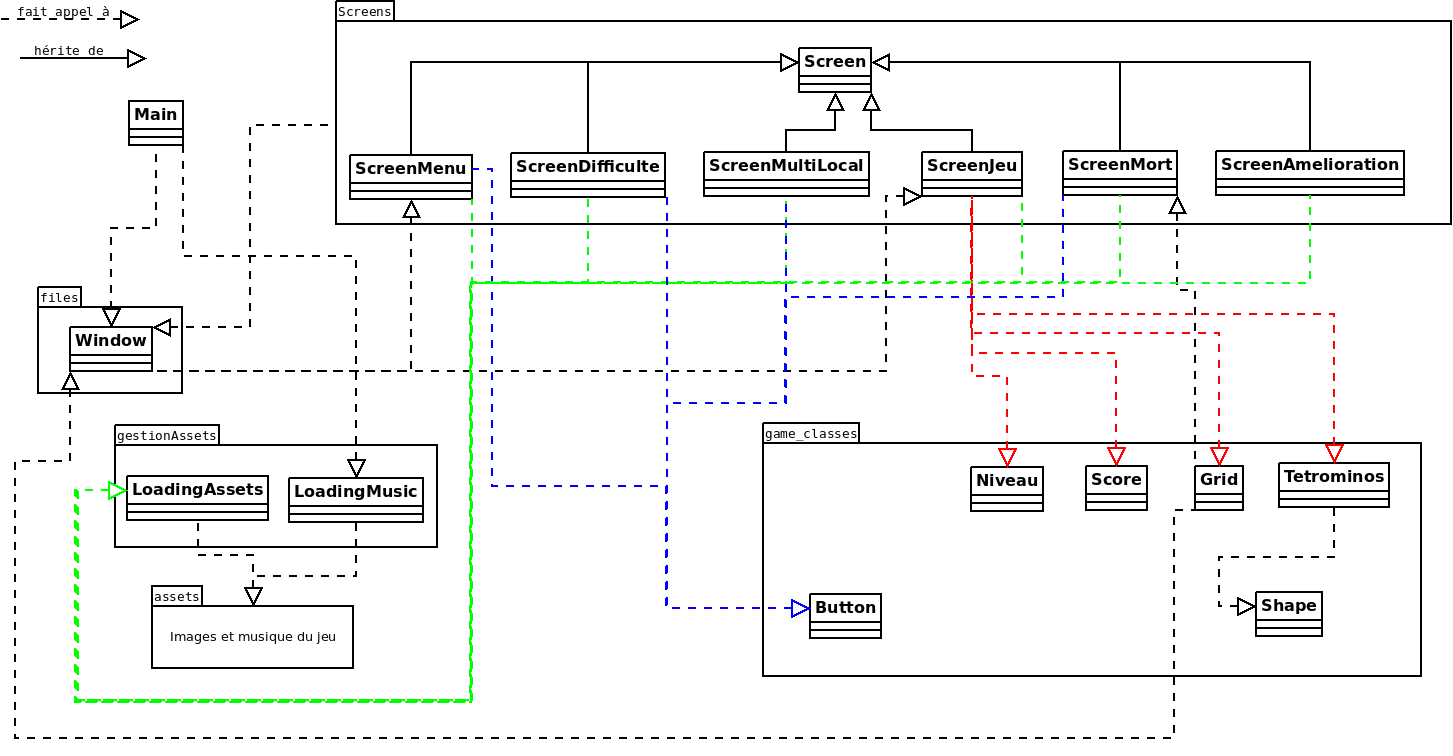
\includegraphics[scale=0.35]{images/diaModClass.png} 
        		\caption{diagramme des modules et des classes}
    		\end{figure}
    		
    		\newpage
            Une fois le mode de jeu sélectionné, on se retrouve dans la classe "ScreenJeu". Cette classe a pour but d'initialiser un certain nombre de fois les éléments que l'on aura besoin pour jouer (les classes Grid,Tetrominos,Score et Niveau) et ainsi créer le nombre d'interface de jeu correspondants, en fonction des choix que l'utilisateur aura fait précédemment dans le menu du jeu. Les classes Grid, Tetrominos, Score et Niveau se chargent des fonctionnalités du Tetris. Une fois le jeu terminé, le jeu nous renvoie sur "ScreenMort". Cette classe à la possibilité de nous renvoyer vers la classe "ScreenMenu" (donc le premier écran du menu principal) ou bien de quitter le jeu (arrêt du programme). 
    	%------------------------------------------------------------------------
        \subsection{Cas d'utilisation}
        %Lorada
            Notre menu est composé de trois écrans (chaque écran correspondant à une classe donc a un fichier dans le dossier "screen"). Au lancement du jeu on a comme premier écran celui de ScreenMenu. Cet écran nous donne le choix entre trois modes de jeu:
            \begin{itemize}
                \item le mode solo, qui constitue une interface de jeu avec une seule grille, un seul affichage de score, un seul affichage de niveau.
                \item le mode multi, qui lui est composé lui-même de deux modes:
                \begin{itemize}
                    \item le mode local, constitué de deux interfaces de jeu avec chacune d'entre elles un score, un niveau et une grille, qui sont à première vue indépendantes mais qui peuvent avoir des interractions entre elles (comme la ligne de malus par exemple). Les deux joueurs jouent sur le même clavier.
                    \item le mode IA, qui se présente de la même manière que le mode local, mais cependant, il s'agit un duel entre un joueur et une IA.
                \end{itemize}
                \item le mode "online", qui est un mode entre deux joueurs s'affrontant sur deux ordinateurs distincts, tout en s'envoyant les informations entre eux en réseau.
            \end{itemize}
            
            \begin{figure}[ht]
                \centering
                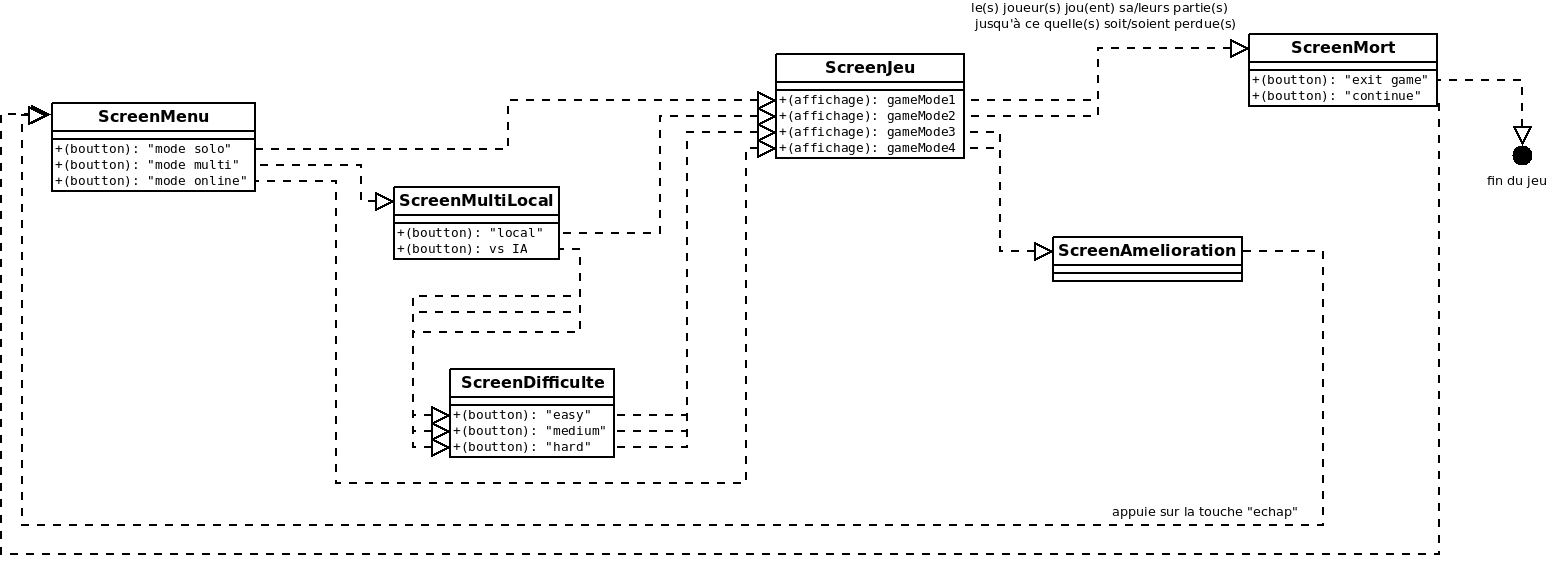
\includegraphics[scale=0.30]{images/diagrammeEvenementiel.png}
                \caption{diagramme événementiel du Tetris}
            \end{figure}
            
            \newpage
            Qu'importe le choix, l'utilisateur se retrouve dans "ScreenJeu" lorsqu'il joue. Dans le cas où le joueur a choisi le mode solo ou le mode local, le(s) joueur(s) joue(nt) au Tetris; si le joueur a choisi le mode contre l'IA ou en ligne, puisque ces modes ne sont pas implémentés, le joueur sera redirigé vers l'écran ScreenAmelioration, affichant une image expliquant que ces modes de jeu ne sont pas disponibles et qu'il s'agit d'une amélioration. Si le joueur appuie sur la touche echap, le programme nous redirige vers le premier écran du menu afin de choisir une autre mode de jeu. 
            \newline 
            \newline 
            Dans le cas où le joueur joue au Tetris, lorsqu'il perd, le programme affiche l'écran de mort, appelé "ScreenMort", lui donnant le choix entre le fait de continuer de joueur et ainsi, sera redirigé vers le premier écran du menu, ou bien de choisir de cliquer sur "Exit game", ce qui lui permettra de quitter le jeu.
        
    %#############################################################################
    \section{Éléments techniques}
        %------------------------------------------------------------------------
        \subsection{Description des fonctionnalités du Tetris}
        
        %Paul
            Pour concevoir un Tetris, on a du réfléchir sur ses fonctionnalités. 
            \newline
  
            \begin{itemize}
                \item Tout d'abord, nous avons du réfléchir à la création des différents Tetrominos dans le jeu. Pour cela, nous avons créé un fichier "Shapes.py" qui contient l'ensemble des pièces du jeu. Chaque pièce est créé sous forme d'un tableau à double entrée (y et x) contenant des "0" et des "1" (les "1" correspondent aux blocs "remplis" d'un Tetrominos, tandis que les "0" correspondent à un bloc vide). Voici un exemple avec la pièce Z:
                
                \begin{figure}[ht]
                    \centering
                    	
\includegraphics[scale=0.8]{images/CapturePiece.png}
                    	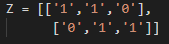
\includegraphics[scale=0.8]{images/PieceCode.png}
                    \caption{La pièce Z et son code}
                \end{figure}
                
                \item Nous avons ensuite stocké toutes les pièces possibles dans un tableau, pour pouvoir les appeler plus tard.
                \item Nous avons ensuite dû penser à créé deux classes: une qui gère les Tetrominos et l'autre la grille
            		
                	\begin{itemize}
                		\item La classe Tetrominos gère les différentes fonctionnalités liées directement aux Tetrominos: leurs créations, leurs affichages, leurs rotations, les différentes collisions, leurs chutes ainsi que leurs déplacements.
                		\item La classe grille gère tout ce qui est lié à la grille du jeu comme la création de la grille, l'implémentation de la pièce dans la grille, la suppression des lignes et la création d'une ligne de malus dans la grille adversaire.
                		\newline
                	\end{itemize}
                \end{itemize}
            
            Nous allons maintenant décrire les fonctionnalités les plus importantes du jeu.
        %------------------------------------------------------------------------ 
        \subsection{Implémentions des fonctionnalités}
        %Paul
        	Nous allons dans un premier temps étudier les fonctionnalités basiques du jeu puis les fonctionnalités spécifiques des	modes multijoueurs.
        	
        	\begin{itemize}
            	\item \underline{les fonctionnalités basiques du jeu:}
            	\newline
            	\begin{itemize}
            	%Paul
            		\item \underline{Création et affichage de la grille:}%Paul
            		On créé un tableau de 10 colonnes et de 20 lignes ne contenant que des zéros>. On gère ensuite l'affichage de la grille: pour se faire, on dessinera un carré d'une taille prédéfini, correspondant à une case du tableau "grille". Si la case contient un zéro, alors elle est vide et affiche un rectangle blanc vide.
            		Si la case est occupée, elle contient un "1" (voir implémentation dans grille) et affiche un rectangle rouge rempli, entouré d'un rectangle blanc vide.
            		\newline
            		\item \underline {Sélection et affichage des Tetrominos:}%Paul
            		Tout d'abord, le programme doit sélectionner deux pièces: une qui sera la pièce actuelle, et l'autre la pièce suivante. Pour cela, nous utilisons la propriété \textit{random.choices} sur le tableau contenant les différentes	pièces possibles du jeu, dans le fichier Shapes. Ensuite, il faut afficher une des pièces dans le milieu de la grille, en haut de celle-ci (ce sera le Tetrominos actuel) et l'autre pièce doit être affichée à coté de la grille du joueur (le Tetrominos suivant). Pour afficher le Tetrominos, on
            		récupère le tableau correspondant à la pièce, sa position dans la grille et on parcours le tableau de la pièce. Si le tableau comporte un "1", alors on affichage un rectangle (violet pour la pièce actuelle et jaune pour la pièce suivante) à la position de la case du tableau, si la case contient un	zéro, on affiche rien.
            		\newline
            		
            		Voici un exemple d'affichage de pièce:
            		
            		\begin{figure}[ht]
                		\centering
                			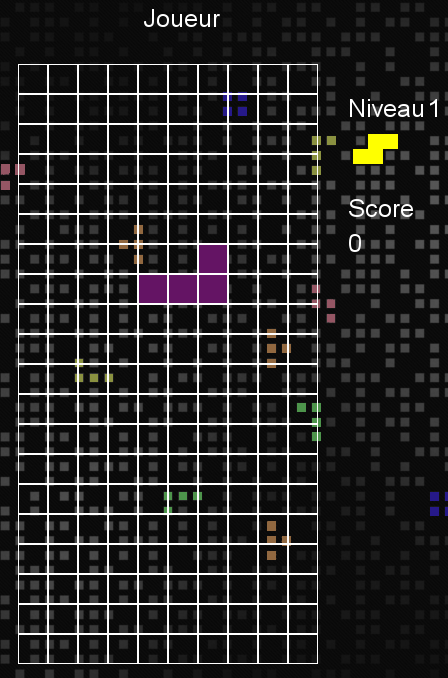
\includegraphics[scale=0.3]{images/Capture.png}
                		\caption{affichage des Tetrominos}
            		\end{figure}
            		
            		%mise à jour du 10 avril
            		\item \underline{Chute des pièces:}%Paul
            		Pour gérer la chute des pièces, nous avons mis en place un système qui se base sur le temps écoulé. C'est à dire qu'à intervalle régulière, le logiciel activera un événement. Dans notre cas, au début du jeu, nous déclenchons l'événement "accélération de la chute" (voir plus bas) toutes les secondes. Cependant, ce temps sera réduit au fur et à mesure des niveaux. Cela simule donc une chute régulière de la pièce jusqu'à ce que la pièce entre en collision avec une autre pièce ou avec le bas du tableau de la grille.
            		\newline
            		
            		%fin des mise à jour du 10 avril
            		\item \underline{Rotation des pièces:} %Paul
            		Cette fonction prend le tableau de la pièce actuelle et récupère son contenu. une fois le contenu récupéré, la fonction fait en sorte de créé un nouveau tableau qui transformera les lignes du tableau en colonnes et vice-versa. Pour finir, on édite le Tetrominos : le tableau du Tetrominos deviens le nouveau tableau créé.
    				\newline
    				Reprenons l'exemple de la pièce Z, voilà ce qui s'affiche lorsque l'on effectue une rotation:
    				
    				\begin{figure}[ht]
                		\centering
                			
\includegraphics[scale=1.2]{images/CapturePiece.png}   
                			
\includegraphics[scale=1.2]{images/rotat.png}
                		\caption{Exemple de rotation}
            		\end{figure}
            		
            		\item \underline{Déplacements:} %Paul
            		On récupère la position du Tetrominos dans la grille et lorsque l'on appuie sur la touche gérant les déplacement (que ce soit vers la droite ou vers la gauche) on modifie la position de pièce (c'est-à-dire de tout les rectangles violets) de façon à ce que la pièce se décale dans la direction souhaitée. 
    				\newline
    				Pour donner l'impression que la pièce se déplace dans la grille, on fait en sorte que la pièce se décale d'un "blocksize" (c'est à dire de la taille d'un bloc correspondant à la taille d'une cellule de la grille).
            		\newline
            		\item \underline{Accélération de la chute:} %Paul
            		Le système est similaire à celui du déplacement des Tetrominos sauf qu'au lieu de se déplacer vers la gauche ou la droite, on fait en sorte que le Tetrominos se décale vers le bas, cela donne l'illusion au joueur que la chute de la pièce est accélérée.
    				\newline
            		\item \underline {Collisions de pièces:} Il y a deux types de collisions dans notre Tetris:
    				\newline
    				
    				\begin{itemize}
            			\item \underline{Collision avec les murs de gauche et de droite:}%Paul
    	
    					Dans un premier temps, nous créons un mur à droite et à gauche de la grille de jeu. Ensuite, nous gérons les collisions avec ces murs: lorsque la pièce rentre en collision avec le mur, nous annulons le mouvement qui est à l'origine de cette collision, cela permet de maintenir la pièce dans la grille
    					\newline
    					
    					\item \underline{Collision avec les pièces et avec le mur du bas:}%Paul
    	
    					Dans un premier temps nous devons créé un mur en bas de la grille et nous devons faire apparaître les pièces dans la grille (voir chapitre "les Tetrominos dans la grille"). Dans un second temps, nous devons gérer la collision de la pièce actuelle avec ce mur du bas et les autres pièces déjà présentes dans la grille. En cas de collision, nous devons alors ajouter la pièce dans la grille et vérifier si l'ajout de cette pièce n'a pas créé de ligne dans notre grille (voir "suppression des lignes") et pour finir, nous devons faire en sorte que le Tetrominos suivant devienne le Tetrominos actuelle et retourne à sa position d'origine (nous devons également choisir un nouveau Tetrominos, choisi aléatoirement qui deviendra le Tetrominos suivant).
    					\newline
            		\end{itemize}
            		
            		\item \underline{insertion des pièces:}%Paul
            		Lorsque le Tetrominos rentre en collision avec le mur du bas ou avec une case occupée de la grille, nous devons intégrer ce Tetrominos à la grille. Pour cela, nous devons récupérer la position du Tetrominos dans la grille. Une fois la position du Tetrominos récupérée, nous devons modifier les cases de la grille où se trouve le Tetrominos pour qu'elles deviennent des cases occupées. Il suffit de modifier les données du tableau de la grille: pour chaque case contenant un bloc du Tetrominos, nous changeons le zéro contenu dans cette case en "1".
    				\newline
    	
    				Voici un exemple d'une grille d'une partie en cours: les cases en rouge dans le jeu sont les pièces déjà présentes dans la grille et nous pouvons voir que chaque case rouge du jeu correspond à une cellule de la grille du jeu contenant un "1".
    
    				\begin{figure}[ht]
                		\centering
    						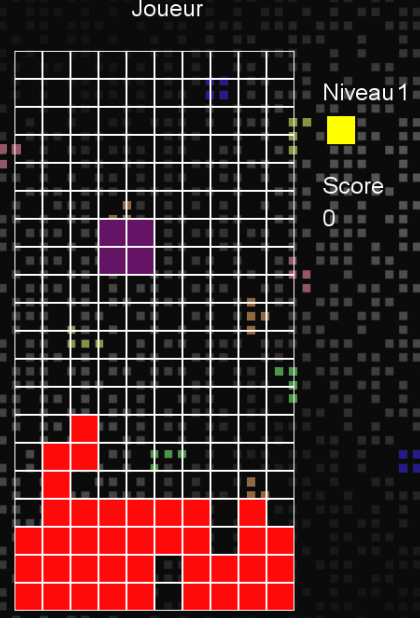
\includegraphics[scale=0.3]{images/Jeu.png}
    						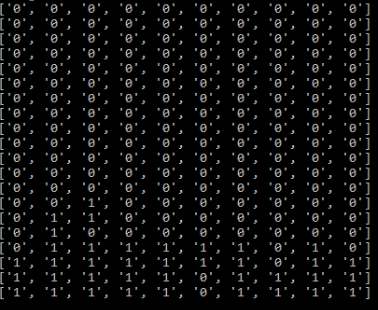
\includegraphics[scale=0.5]{images/console.png}
    					\caption{Grille de jeu et affichage de la console}
            		\end{figure}
            		
            		\item \underline{Suppression des lignes:} %Paul
            		Si un joueur arrive à remplir toute une ligne avec les Tetrominos, nous devons faire en sorte que cette ligne disparaisse. Pour cela, à chaque fois qu'un nouveau Tetrominos est ajouté à la grille, nous parcourons la grille et nous regardons si une ligne de la grille est rempli de "1". Si c'est le cas nous supprimons cette ligne du tableau et nous la remplaçons par une nouvelle ligne au début du tableau tout en ajoutant des points au joueurs.
            		\newline
            		
            		\item \underline{Gestion des niveaux:} %Lorada
            		Le joueur augmente d'un niveau lorsque celui-ci à supprimé un certain nombre de lignes (dans notre programme, cela correspond à dix lignes). La valeur du niveau a une conséquence directe avec la vitesse de chute (celle-ci est augmentée au fur et à mesure du niveau) ainsi que la valeur du score (le score obtenu en supprimant une ligne est de plus en plus grand en fonction du niveau).
            		
            		\item \underline {Gestion du score:} %Lorada 
            		Le score est calculé de manière suivante: \textbf{(25*n+100*(n-1))*niveau}
            		où n correspond au nombre de lignes qui ont été détruites sur le coup.
            		\newline
            		Dans le cas où nous détruisons une seule ligne sur le coup, le calcul est celui-ci: \textbf{(25*n)*niveau}, c'est-à-dire que:
            		\begin{itemize}
            		    \item pour le niveau 1, le score est de 25 points supplémentaires,
            		    \item pour le niveau 2, le score est de 50 points supplémentaires,
            		    \item pour le niveau 3, le score est de 75 points supplémentaires, et ainsi de suite.
            		 \end{itemize}
            		 
            		Cependant, lorsque le joueur réalise un combo, le score doit être plus important. Le combo correspond donc à \textbf{100*(n-1)} dans le calcul. De ce fait, lorsqu'il n'a pas de combo (une seule ligne supprimée sur le coup), le résultat de ce calcul est nul. Lorsqu'il y a réalisation d'un combo, on a, à la fois le calcul du score de base (donc \textbf{(25*n)*niveau}) ainsi que le calcul du combo:
            		\begin{itemize}
            		    \item pour deux lignes de supprimées en même temps: \textbf{100*(2-1)} = 100 points de combo rajoutés
            		    \item pour trois lignes de supprimées en même temps: \textbf{100*(3-1)} = 200 points de combo rajoutés
            		    \item pour quatre lignes de supprimées en même temps: \textbf{100*(4-1)} = 300 points de combo rajoutés 
            		\end{itemize}
            		Il n'y a pas moyen de supprimer plus de quatre lignes en même temps dans un Tetris. 
            	    \newline
            	    
            		\item \underline{fin du jeu:} %Lorada
            		La fin du jeu est défini au moment où la case à la position x = 5 et y = 0 , (c'est-à-dire à la cinquième case tout en haut de la grille), contient un "1". On a choisi cette position car c'est la position à laquelle un nouveau Tetrominos se positionne au départ. Si cette case contient un "1", alors il est impossible de continuer de jouer puisque le Tetrominos n'aura plus la possibilité d'avoir une position de départ.
            	\end{itemize}
            	
            	\item \underline {les fonctionnalités spécifiques au mode multijoueurs:}%Paul
            	\newline		
            	\begin{itemize}
            		\item \underline {Gestion de la ligne de malus:} Nous avons vu plus haut, ce que se passait si un joueur remplissait une ligne dans sa grille. Dans le mode multijoueurs, lorsqu'un joueur réussit à compléter une ligne, cela créé un malus pour le joueur adverse. Cette fonctionnalité supprime la première ligne de la grille du premier joueur et rajoute une ligne de malus au joueur adverse (il s'agit d'une ligne qui est composé de neuf "1" et un "0" qui seront réparti aléatoirement, c'est à dire que le joueur adversaire verra apparaître en bas de sa grille une ligne contenant neuf casé occupées (neuf cases rouges et une case vide)).
            		\newline
            		        		
            		\item \underline {Affichage de plusieurs interfaces de jeu:}	%Lorada
            		L'interface de jeu d'un joueur est constitué de ces éléments:
            		\begin{itemize}
            		    \item l'affichage d'une grille
            		    \item l'affichage d'un Tetrominos qui puisse être contrôlé
            		    \item l'affichage du Tetrominos suivant
            		    \item l'affichage du score
            		    \item l'affichage du niveau
            		\end{itemize}
            		
                Pour cela, nous avons besoin d'appeler les classes correspondantes pour chacun de ces éléments. On fait donc appel au constructeur de chacune des classes le nombre de fois que nous en avons besoin (ici, c'est dans le cas où le joueur est seul, ainsi que pour le joueur 1 et le joueur 2 dans le mode multijoueurs). 
                
                \begin{figure}[ht]
                    \centering
                    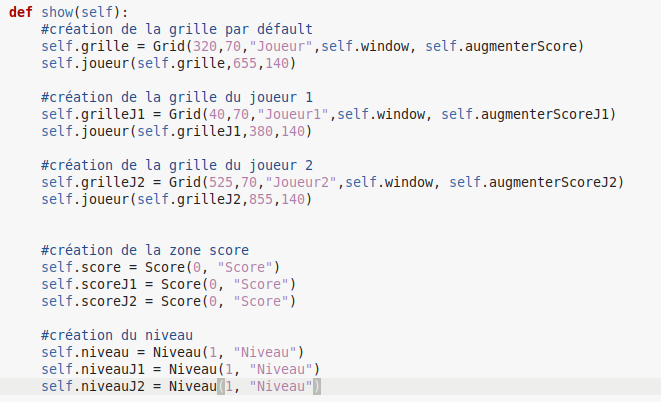
\includegraphics[scale=0.5]{images/appelConstr.png}
                    \caption{Appel des constructeurs des classes}
                \end{figure}
                
                \newpage
                Ensuite, en fonction du mode de joueur sélectionné, nous appelons la fonction \textit{update} de la classe Grid, qui se charge mettre à jour tout le statut du jeu (les Tetrominos, la grille, etc.)
                \newline
                Le mode de jeu est défini par une variable qui est envoyé par l'écran précédent. Cette variable déterminera l'affichage, le nombre de joueur, et toute les actions propres au jeu.
                
                 \begin{figure}[ht]
                    \centering
                    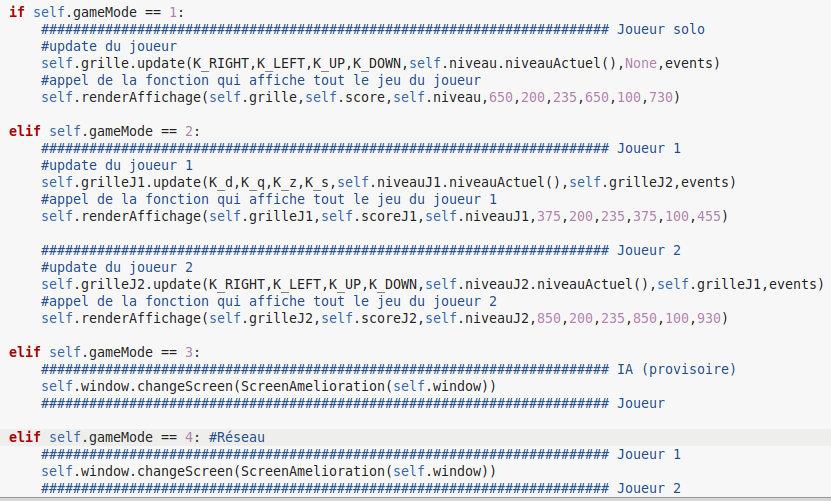
\includegraphics[scale=0.5]{images/gameMode.png}
                    \caption{choix du mode de jeu}
                \end{figure}
                
                Étant donné que le mode qui est contre une IA ainsi que le mode en réseau ne sont pas disponibles (seulement une réflexion sur ces modes ont été faites), nous avons fait en sorte que le jeu nous renvoie vers l'écran d'amélioration, comme expliqué précédemment.
                
            	\end{itemize}
            		
        	\end{itemize}
        	\newpage
        %------------------------------------------------------------------------ 
        \subsection{Algorithmes spécifiques}
            %ici: algorithmes: Paul      	
    		\begin{algorithm}
     			\centering
     			\begin{algorithmic}[1]
      				\STATE \textbf{Variables:} Grille(tableau),nombre de colonnes, nombre de ligne
      				\STATE \textbf{Programme:} Création de la grille de jeu
      				\STATE Récupérer le nombre de colonnes et le nombre de lignes
      				\FOR{i allant de 1 au nombre de lignes }  
      					\STATE  Ajouter un tableau dans le tableau Grille
      					\FOR{j allant de 1 au nombre de colonnes}
      						\STATE Ajouter un "0" dans le tableau du tableau Grille
      					\ENDFOR
      				\ENDFOR
      				\STATE Renvoyer la grille
     			\end{algorithmic}
     			\caption{Algorithme de la création de la grille du jeu}
     		\end{algorithm}
    			     	
            \begin{algorithm}%Paul
     			\centering
     			\begin{algorithmic}[1]
      				\STATE \textbf{Variables:} pièce(tableau 2D),largeur de la pièce,longueur de la pièce
      				\STATE \textbf{Programme:}Rotation des pièces
      				\STATE Événement "retourne pièce" activé
      				\STATE Récupérer la hauteur de la pièce(longueur de la première dimension du tableau pièce)
      				\STATE Récupérer la largeur de la pièce(longueur de la deuxième dimension du tableau pièce)
      				\STATE Créer un tableau 2D "pièce retournée"
      				\FOR {i allant de 1 à largeur de la pièce }
      					\STATE Créé un tableau dans le tableau "pièce retournée" contenant x "0" (x = hauteur de la pièce)
      				\ENDFOR
       					\FOR{i allant de 1 à largeur de la pièce}
        					\FOR{x allant de 1 à largeur de la pièce}
         						\STATE La case de coordonnées[x,y] du tableau "pièce retournée" prend la valeur de la case de 									coordonnées[y,(largeur de la pièce-1-x] du tableau pièce
        					\ENDFOR
       					\ENDFOR
      				\STATE Le tableau pièce deviens le tableau pièce retournée
      				\STATE Rafraîchi l'affichage de la pièce
     			\end{algorithmic}
     			\caption{Algorithme de la rotation des pièces}
    		\end{algorithm}	
            
            
     		\begin{algorithm}%Paul
     			\centering
     			\begin{algorithmic}[1]
      				\STATE \textbf{Variables:} pièce(tableau 2D),position de la pièce,mur de gauche et mur de droite, position du 					mur de gauche et du mur de droite, grille adverse(tableau 2D)
      				\STATE \textbf{Programme:} Collision de la pièce avec le mur de gauche ou le mur de droite
      				\STATE Déplacement de la pièce vers la gauche ou déplacement vers la droite
      				\STATE Récupérer la nouvelle position de la pièce, le position du mur de gauche et du mur de droit
      					\IF{La position de la pièce rentre en collision avec la position du mur de gauche ou du mur de droite}
      						\STATE	Annuler le mouvement
      					\ENDIF
     			\end{algorithmic}
     			\caption{Algorithme de la collision de la pièce avec le mur de gauche ou le mur de droite}
     		\end{algorithm}
     		
     		\begin{algorithm}%Paul
     			\centering
     			\begin{algorithmic}[1]
      				\STATE \textbf{Variables:} pièce(tableau 2D),position de la pièce,mur du bas, position du mur du bas, grille(tableau 2D),pièce présente dans la grille, position des pièces de la grille, pièce suivante
      				\STATE \textbf{Programme:} Collision de la pièce avec le mur du bas ou les pièces présentes dans la grille
      				\STATE Chute et/ou accélération de la pièce
      				\STATE Récupérer la nouvelle position de la pièce, le position du mur du bas et du mur des pièces présente 						dans la grille
      					\IF{La position de la pièce rentre en collision avec la position du mur du bas ou des pièces de la grille}
      						\STATE	Ajouter la pièce dans la grille
      						\IF{Une ligne de la grille est pleine}
      							\STATE Supprimer la ligne pleine de la grille
      							\STATE Ajouter une nouvelle ligne au début de la grille
      							\IF{mode multijoueurs}
      								\STATE Supprimer la première ligne de la grille adverse
      								\STATE Ajouter une ligne malus quasiment pleine à la grille du joueur adverse 
      							\ENDIF
      						\ENDIF
      						\STATE La pièce deviens la pièce suivante
      						\STATE La pièce est renvoyer à sa position de départ
      						\STATE Tirer une nouvelle pièce suivante
      					\ENDIF
     			\end{algorithmic}
     			\caption{Algorithme de la collision de la pièce avec le mur du bas ou les pièces de la grille}
     		\end{algorithm}
    	%###########################################################################	
        \newpage
        \section{Pistes et réflexion de certains aspects}
        %---------------------------------------------------------------------------
        \subsection{Réflexion sur la conception de l'IA}
        %Hugues
            \subsubsection{Création d'une IA - les prémisses}

                La création d'une IA pour Tetris aura sans doute était l'une des choses les plus dures que nous ayons eu à faire, même si nous n'avons pas pu l'ajouter dans la version finale du projet, il est important d'expliquer comment elle aurait été faite si nous avions eu le temps de la finir.
                
                Au tout début nous avions pensé à une IA qui, en fonction de trois nombres générés aléatoirement à chaque apparition de pièce devait définir les mouvements gauche, droite et rotation de cette pièce, mais l'IA s'avérait inefficace et ne réussissant pas à compléter une seule ligne, l'idée fût abandonnée.

            \subsubsection{Une deuxième IA}
                Lors d'une discutions avec un élève de L2 nous lui avons parlé de notre problème et il nous a conseillé de nous renseigner sur un algorithme du nom de "Min-max", cet algorithme permettrait de générer
                un arbre de jeu qui permettrait de trouver la meilleure action à faire en fonction de certains facteurs. \newline 
                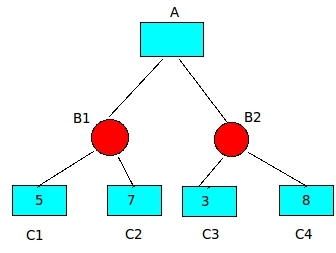
\includegraphics[scale=0.6]{images/minmax.jpg}

            \subsubsection{Application de l'algorithme min-max}

                Tout d'abord nous devions parcourir la grille à chaque fois qu'une pièce de l'IA apparaissait  pour voir l'avancement de la partie, comme le but du Tetris est de compléter des lignes il a donc fallu ajouter un score interne au bot.\newline\\ Chaque case de la dernière ligne représentant un point pour le bot, il lui faudra donc trouver la meilleure position pour prendre le plus de case possible et donc avoir le plus de point possible et de cette manière, le bot cherchera toujours à compléter des lignes, et c'est donc là que l'algorithme min-max intervient.
                
                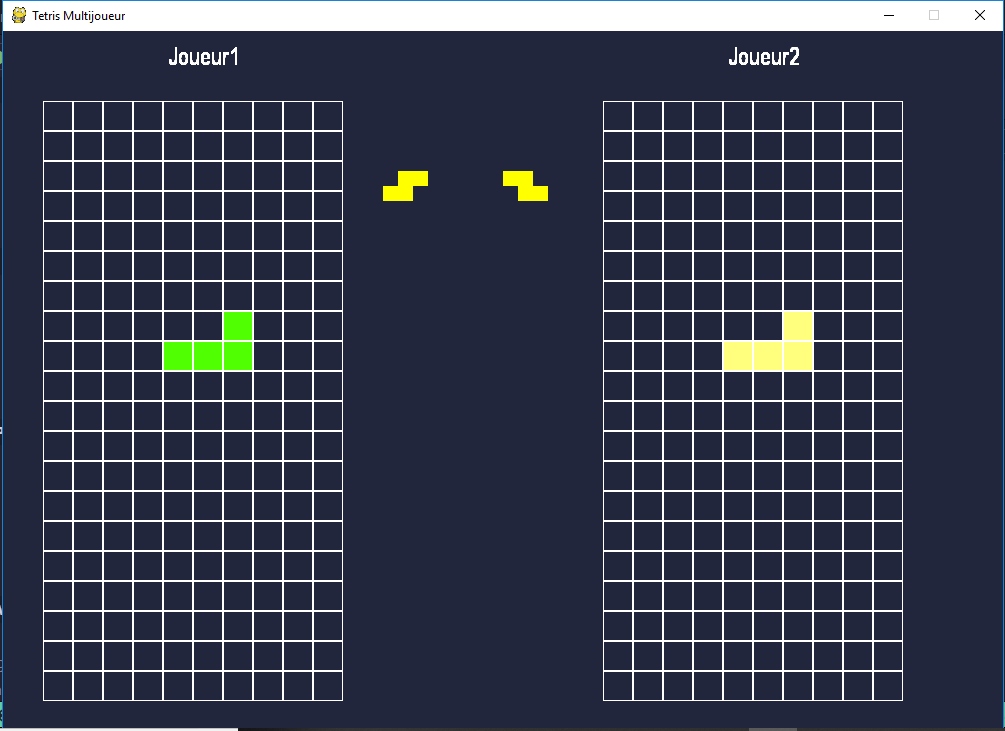
\includegraphics[scale=0.6]{images/grille.png}
                
                L'algorithme va donc tester chaque coup et garder le meilleur tant qu'elle n'aura pas trouvé un coup qui rapporte un meilleur score.\newline
                Puis, à chaque nouvelle pièce, on répétera l'opération permettant de trouver la meilleure "solution", l'algorithme cherchera le meilleur déplacement et ainsi jouera.
        %----------------------------------------------------------------------------
        \subsection{Réflexion sur le réseau}
        % Willy
            Pour le réseau il fallait commencer par créer un serveur. Pour fonctionner, il fallait dire sur quel port de l'ordinateur écouter. Ensuite il fallait lui indiquer qu'il était l’hôte du réseau. On a alors créée un client capable de se connecter au serveur. Pour se faire on a renseigné le port utilisé par le serveur et son adresse IP. Cependant cela n'a pas fonctionné car il faut que le serveur et le client soient connectés sur le même réseau informatique.\\ Une fois que le serveur est lancé, il nous informe sur quelle port il écoute.

            \begin{figure}[ht]
                \centering
                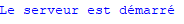
\includegraphics[]{images/serveur.png}
            \end{figure}
            
            Lorsqu'un client se connecte au serveur il y a un message.
            
            \begin{figure}[ht]
                \centering
                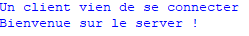
\includegraphics[]{images/client_conecter.png}
            \end{figure}
            
            Tandis que sur le client on voyait

            \begin{figure}[ht]
                \centering
                
\includegraphics[]{images/client.png}
            \end{figure}
            
            Pour le réseau on s'est aidé du site Openclassrooms \url{https://openclassrooms.com/fr/}. On a également fait des recherche sur le réseau et si on avais pus le rajouter dans le projet alors il aurait suffit de démarrer le serveur en même temps que le jeu et ensuite il aurais fallu également créé un client capable de se connecter au serveur en lançant le jeu. Mais le réseau de la FAC bloque la connexion entre les ordinateurs.
        
        
    %###########################################################################
    \section{Expérimentation et usage}
        \subsection{Visuel de l'accès au jeu}
            %Lorada
            Tout d'abord, nous avons besoin de récupérer le projet sur SVN lorsque celui-ci n'est pas sur la machine. Pour cela, nous avons besoin de faire un "checkout". Sur Linux, il faut inscrire cette commande dans le terminal: \textbf{svn checkout https://forge.info.unicaen.fr/svn/jeu-de-Tetris --username=NUMETU} dont NUMETU correspondant à un numéro étudiant d'une personne présente dans le projet. Ensuite, tout le dossier du projet est importé sur la machine.
            
            Une fois cette étape réalisée, il faut cliquer sur jeu-de-tetris, ouvrir le terminal et lancer le programme en lançant la main avec la commande ci-dessous:
            
            \begin{figure}[ht]
                \centering
                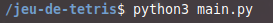
\includegraphics[scale=0.75]{images/lanceMain.png}
                \caption{commande pour lancer le jeu}
            \end{figure}
            
            On se retrouve alors sur cet écran: 
            
            \begin{figure}[ht]
                \centering
                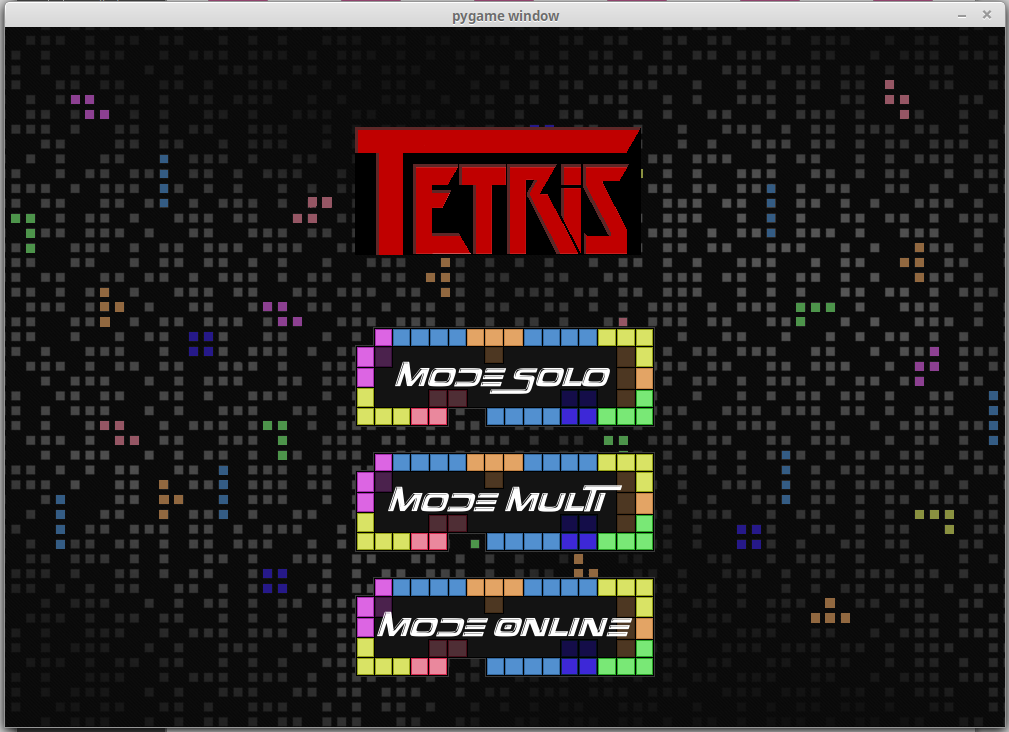
\includegraphics[scale=0.25]{images/ecran1.png}
            \end{figure}
            On a alors le choix entre le mode solo, qui, lorsque l'on clique dessus, nous amène sur cet écran. Le joueur peut alors jouer tout seul au Tetris.
            
            \begin{figure}[ht]
                \centering
                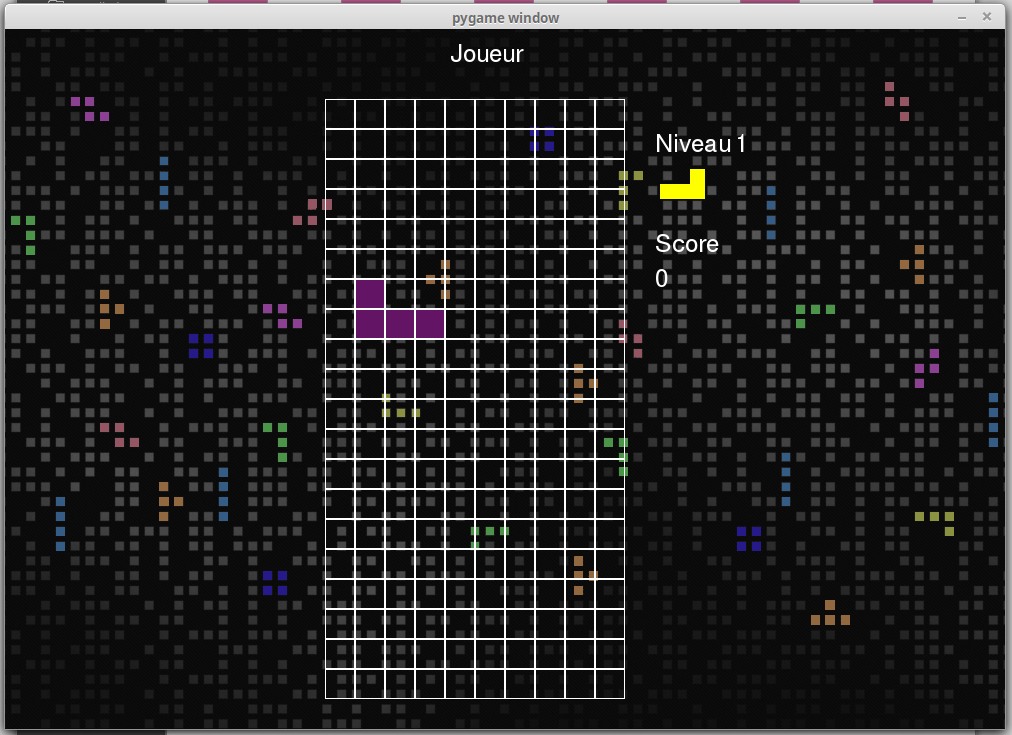
\includegraphics[scale=0.25]{images/jeuSolo.png}
            \end{figure}
            \newpage
            Dans le cas où le joueur séléctionne le mode multijoueurs, il se retrouve sur cet écran:
            
            \begin{figure}[ht]
                \centering
                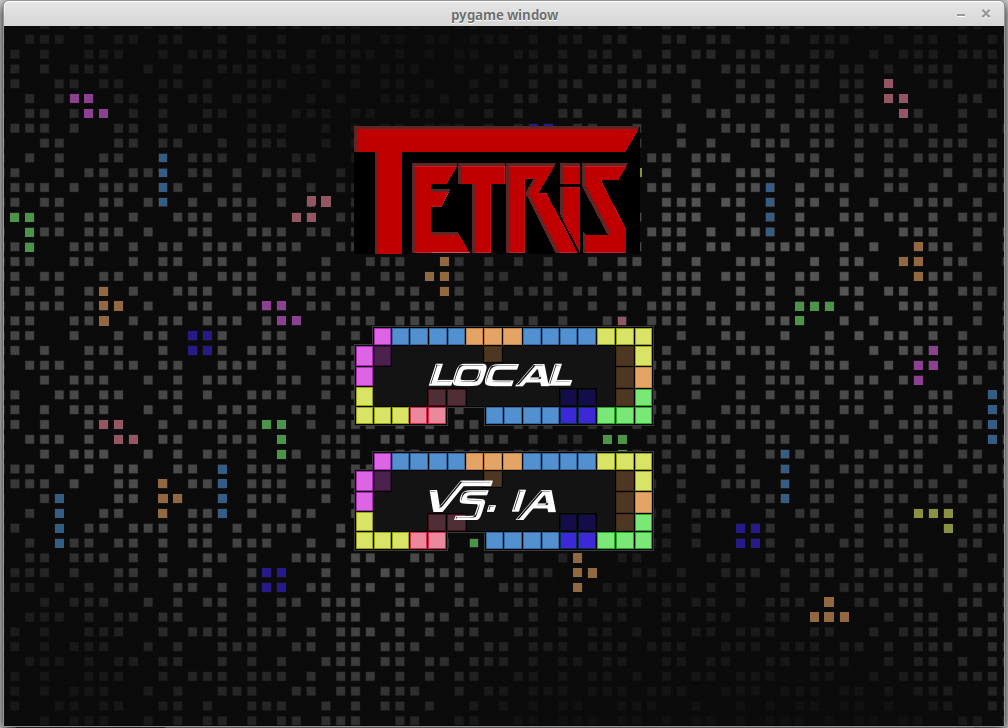
\includegraphics[scale=0.25]{images/ecranMulti.png}
            \end{figure}
            
            Le joueur peut choisir entre le fait de joueur à deux joueurs en local ou contre une IA. Dans le cas où il choisi le premier choix, on se retrouve sur cet écran:
            
           
            \begin{figure}[ht]
                \centering
                 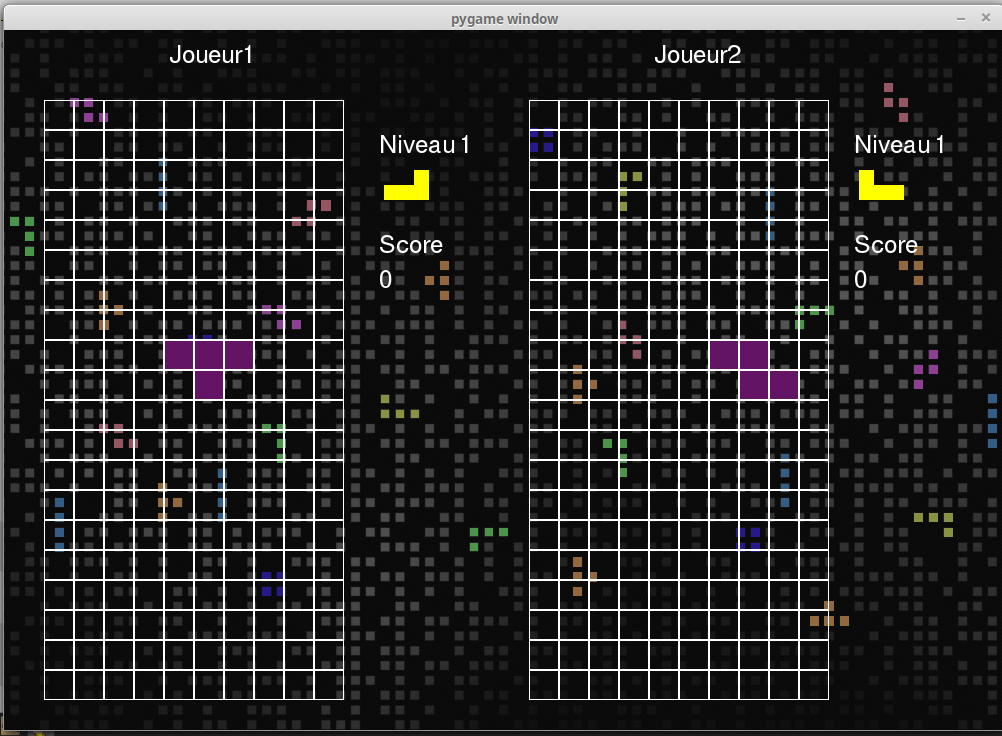
\includegraphics[scale=0.25]{images/jeu2J.png}
            \end{figure}
            
            \newpage
            Si le joueur choisi le mode contre une IA, il a le choix entre trois modes de difficulté (correspondant à une IA plus ou moins sophistiquée): 
            
            
            \begin{figure}[ht]
                \centering
                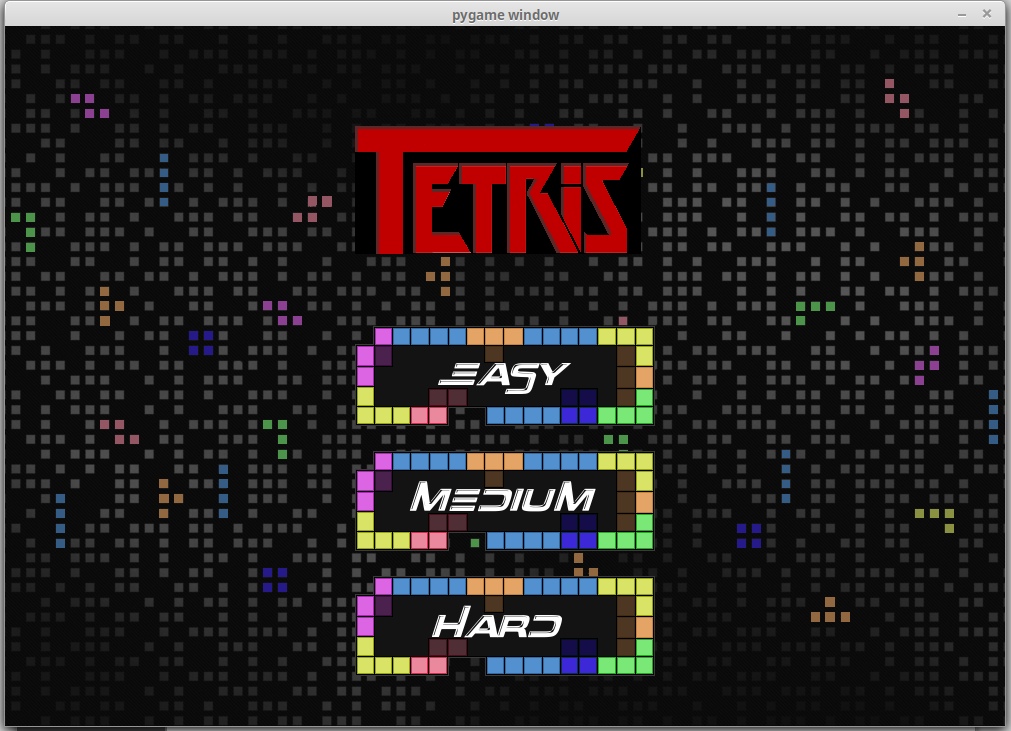
\includegraphics[scale=0.25]{images/jeuDiff.png}
            \end{figure}
            
            
            Une fois le mode de difficulté choisi, le joueur est sur cet écran: 
            
            \begin{figure}[ht]
                \centering
                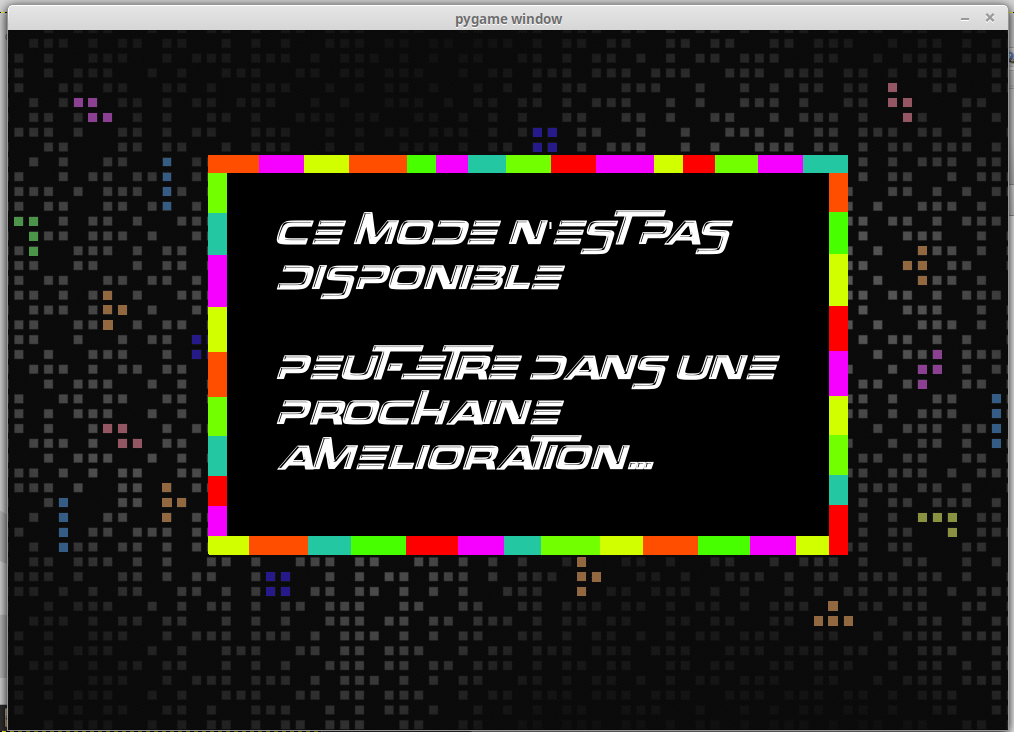
\includegraphics[scale=0.25]{images/jeuAme.png}
            \end{figure}
            
            Comme précisé précédemment, le mode en ligne et celui contre une IA n'étant pas encore présents, il est normal d'arriver sur cet écran affichant ce message. Cet écran s'affichera également si nous sélectionnons le mode en ligne. 
            
        \newpage
        \subsection{Visuel du Tetris}
            Voici quelques images du jeu en lui-meme dans le mode solo:
            
            \begin{figure}[ht]
                \centering
                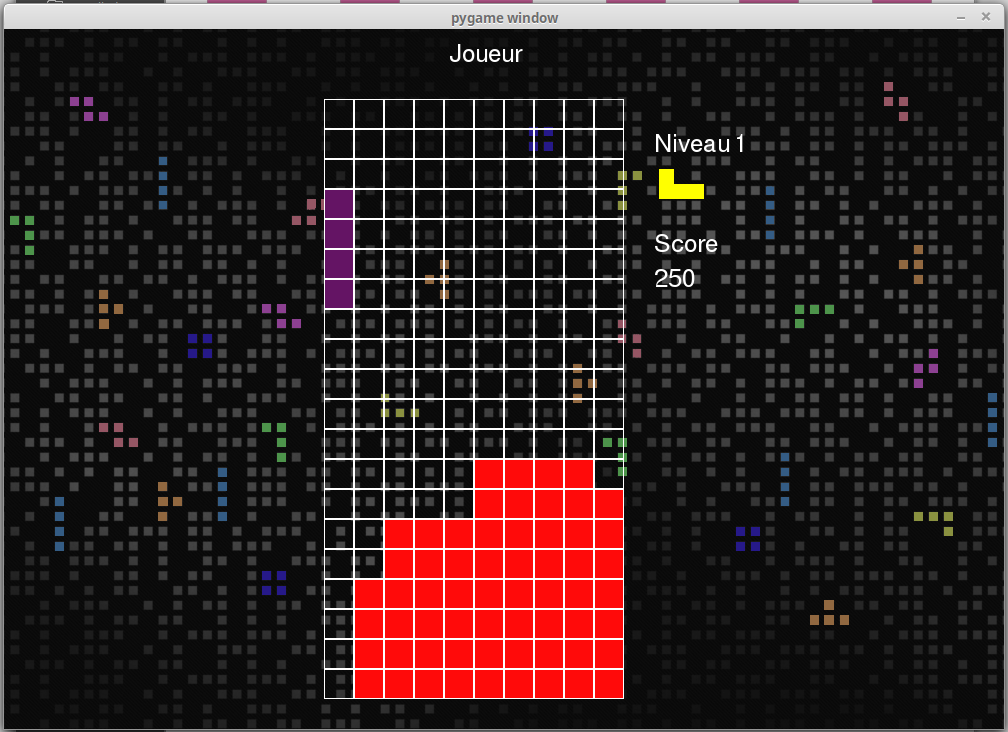
\includegraphics[scale=0.25]{images/jeu3.png}
                
            \end{figure}
            
            \begin{figure}[ht]
                \centering
                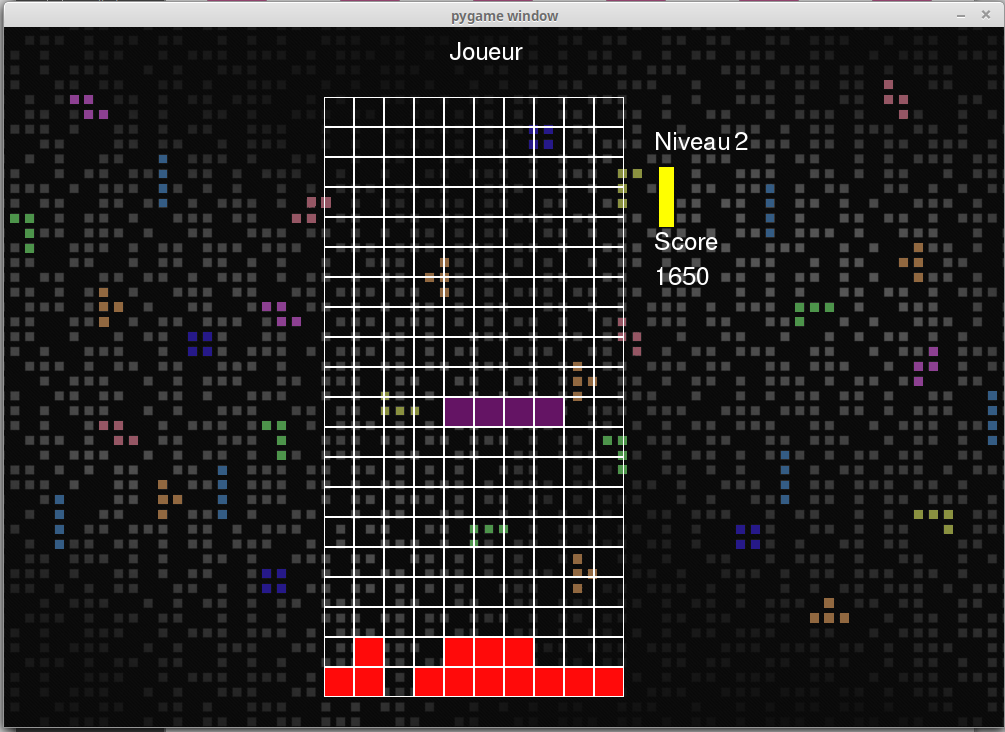
\includegraphics[scale=0.25]{images/jeu1.png}
            \end{figure}
            
            \begin{figure}[ht]
                \centering
                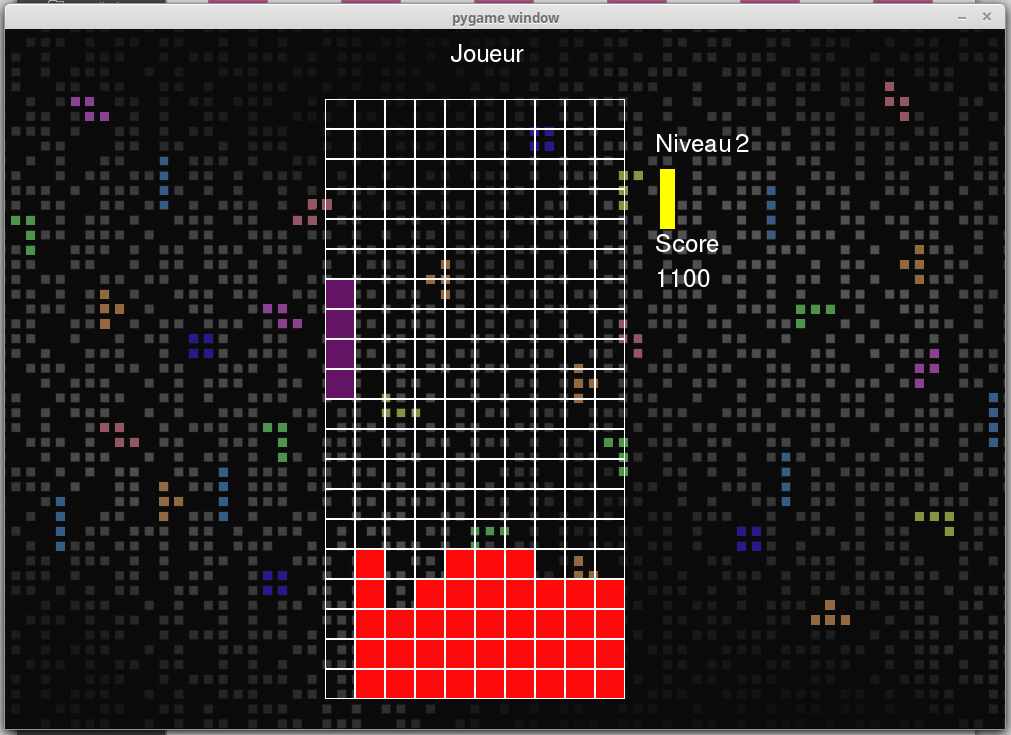
\includegraphics[scale=0.25]{images/jeu4.png}
            \end{figure}
            \newpage
            Anisi que dans le mode multijoueurs:
            
            \begin{figure}[ht]
                \centering
                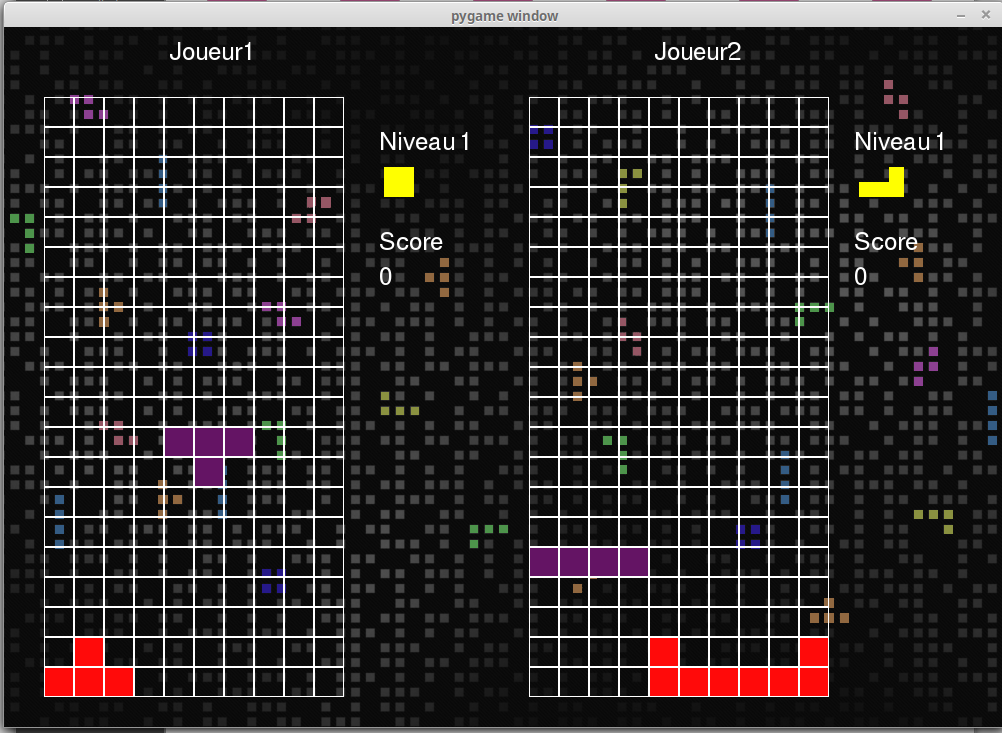
\includegraphics[scale=0.25]{images/jeuM1.png}
                \caption{Capture d'écran avant que le joueur 2 supprime une ligne}
            \end{figure}
            
            \begin{figure}[ht]
                \centering
                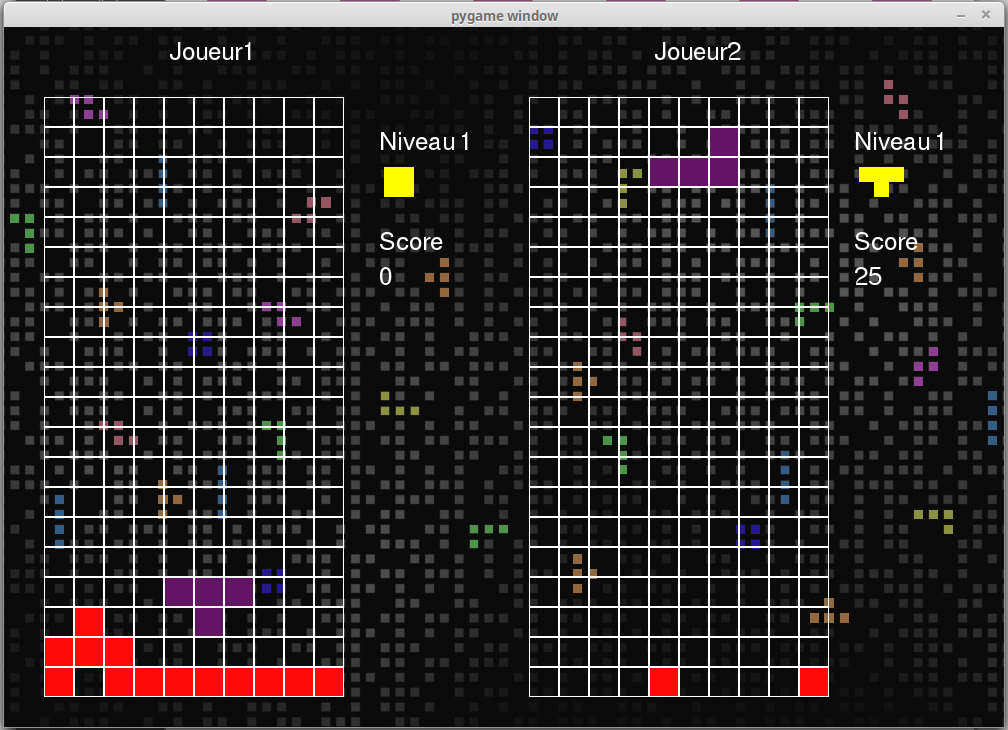
\includegraphics[scale=0.25]{images/jeuM2.png}
                \caption{Capture d'écran après que le joueur 2 supprime une ligne: le joueur 1 ayant reçu une ligne de malus}
            \end{figure}
          
        
    %###########################################################################
    \newpage
    \section{Conclusion}
            Pour conclure, nous pouvons donc dire que nous avons rempli la plupart de nos objectifs: le Tetris est fonctionnel pour le mode solo et multijoueurs local mais nous n'avons malheureusement pas réussi à réaliser l'Intelligence artificielle ni le mode multijoueurs en réseau. La plupart des fonctionnalités sont pleinement opérationnelles (que ce soit la création et l'affichage de la grille, la gestion de la chute des pièces, leur implémentation dans la grille, la suppression des lignes , l'ajout d'une ligne de malus et la gestion du score et des niveaux). Nous pouvons néanmoins remarqué certains bugs à certains endroits du jeu, notamment au niveau des collisions: par exemple, lorsque l'on appuie plein de fois sur la touche gauche ou droite au moment où tetrominos se trouve près de la grille, on peut remarquer rapidement la pièce sortir de la grille avant de retourner dans la grille. Nous pouvons également voir un autre bug au niveau de l'implémentation des pièces, parfois, une case vide de la grille se rempli lorsqu'un Tetrominos est ajouté dans la grille et qu'il reste une case vide en dessous du Tetrominos inséré dans la grille.
     %###########################################################################
       \section{Les pistes d'améliorations}
        %ici: proposition d'amélioration
        	Nous pourrions ajouter de nouvelles fonctionnalités, notamment dans les modes multijoueurs pour rendre le jeu d'avantage tendu, par exemple, nous pourrions proposer des fonctionnalités permettant d'intervertir le Tetrominos en cours des deux joueurs en échange d'une certaine somme de points. Nous pourrions également essayer de rendre le jeu plus équilibré en imposant un malus au meilleur des deux joueurs si l'écart entre le score des deux joueurs devient trop important.
        	\newline
        	
        	Nous pourrions aussi ajouter un mode de jeu un joueur dans lequel une grille serait déjà en partie rempli et le joueur devrait alors tenter de faire disparaitre tout les Tetrominos déjà présent dans la grille pour gagner.
    
    %#############################################################################
    \newpage
    \section{Sources}
    	\begin{itemize}
    		\item le lien menant vers la première partie du tutoriel : \url{https://www.youtube.com/watch?v=uoR4ilCWwKA}
    		\item le lien menant vers la bibliothèque pygame : \url{http://www.pygame.org/docs/}
    	\end{itemize}

\end{document}